\section{Introduction}
\label{sec:introduction}

% state the learning objective 
\par In this laboratory assignment we study the circuit
shown in Figure~\ref{fig:circuit}, which functions as a Band-Pass Filter
circuit. The report is divided in two main sections.

We started with the simulation of the circuit using the software
\textit{Ngspice}.
Afterwards we proceeded with the theoretical analysis of the circuit,
using nodal analysis.
This procedure is explored in section ~\ref{sec:analysis};
We used the software \textit{Octave} to solve the derived systems
of equations and to plot solutions.
Subsequently we compared the results of the simulation with the
theoretical results. This is described in section ~\ref{sec:simulation}.
Finally, the conclusions of this study are indicated in
Section~\ref{sec:conclusion}.

\begin{figure}[ht] \centering
    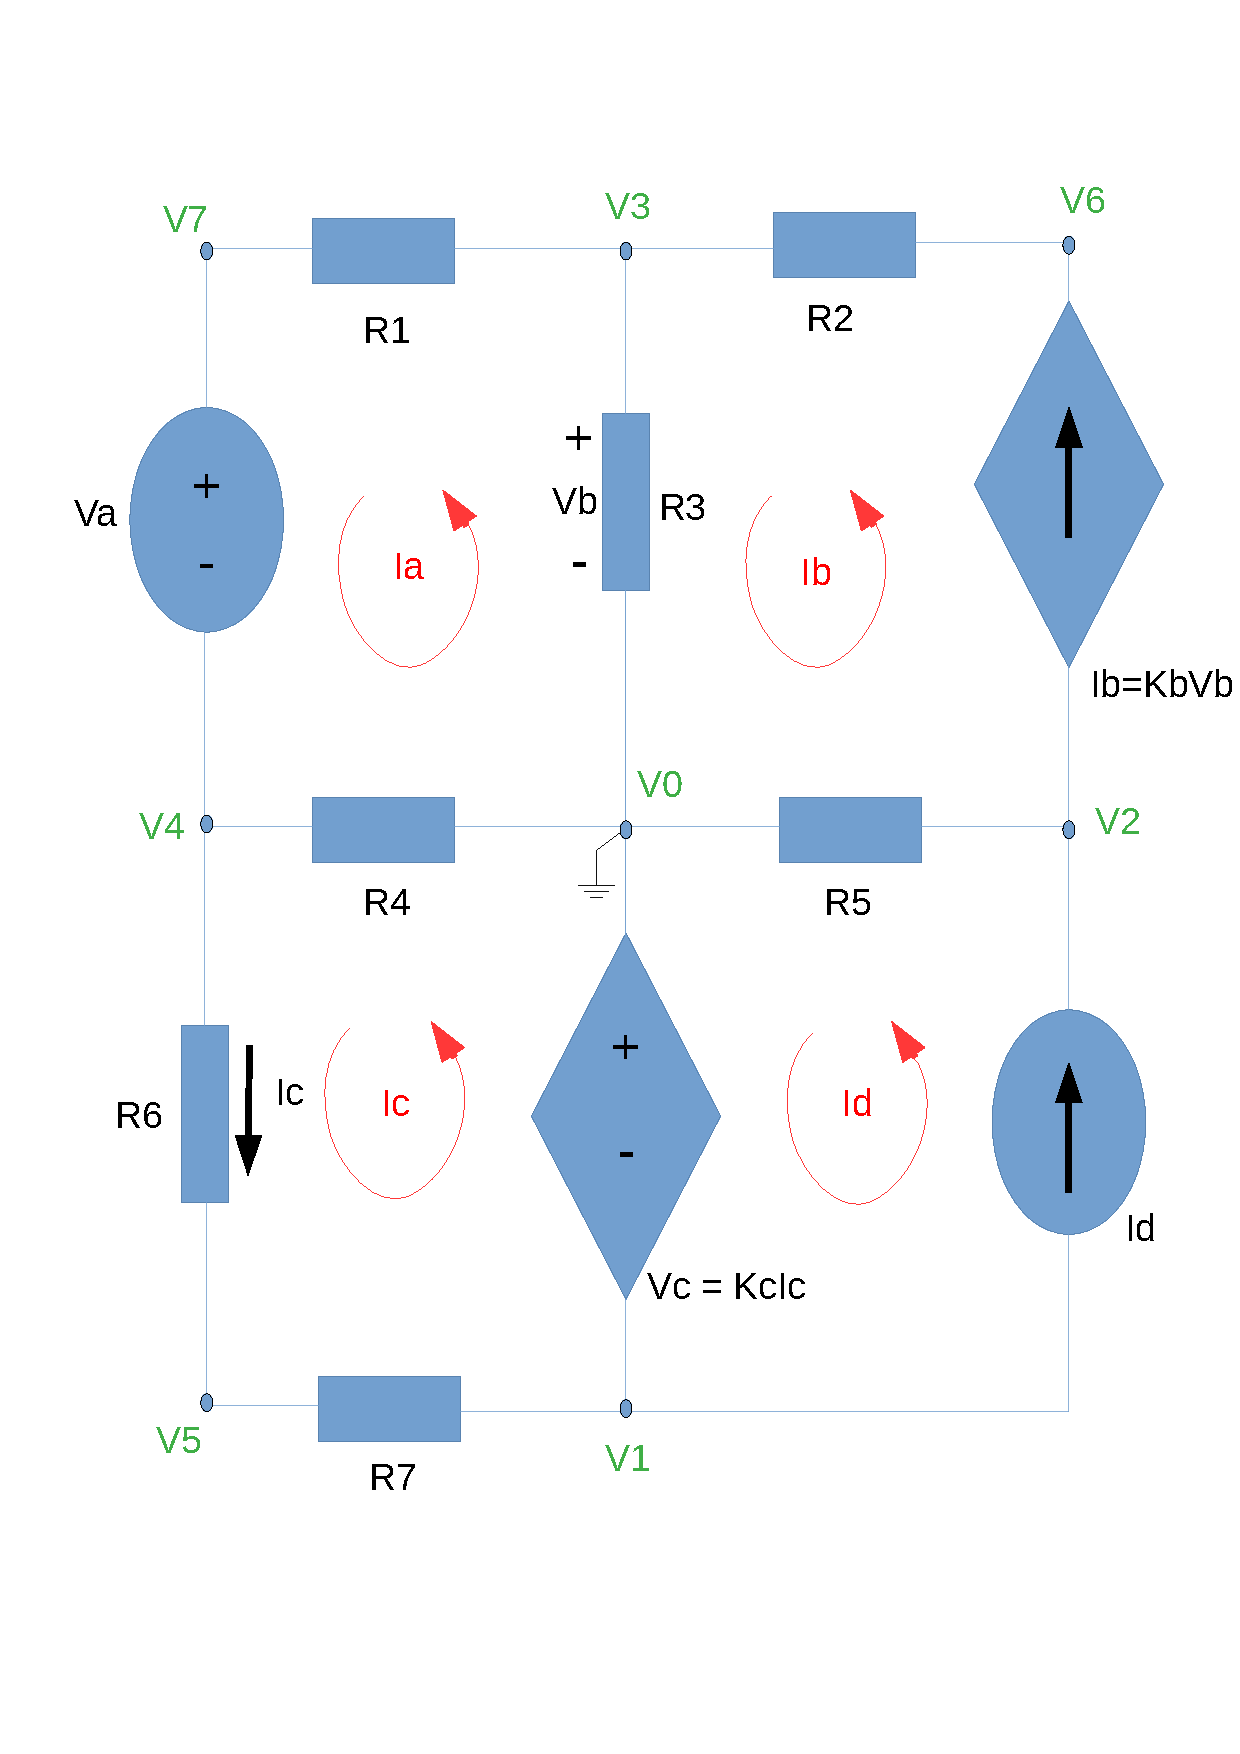
\includegraphics[width=0.6\linewidth]{circuito_tcfe.pdf}
    \caption{Circuit}
    \label{fig:circuit}
\end{figure}

